\section{The Kubernetes Scheduler} \label{section:background_scheduler}

A scheduler on a Kubernetes cluster is a component that watches for newly
created Pods that have no node assigned. For every Pod the scheduler discovers,
the scheduler becomes responsible for finding the best node for that Pod to run
on. In this section, we will present the background needed to understand how
scheduling occurs.

\subsection{Scheduling Fundamentals} \label{section:scheduling-fundamentals}

\paragraph*{Multiple schedulers}

A \textit{scheduler} is a component on a Kubernetes cluster that assigns a node
for each Pod to run on. Kubernetes clusters ship with the default scheduler,
namely \co{kube-scheduler}, which runs as part of the control plane. However,
multiple schedulers may run on a cluster; in this case, each Pod must specify
the scheduler's name that shall handle it by setting its \co{spec.schedulerName}
field to the name of the preferred scheduler. If a scheduler name is not
explicitly specified, the Pod will be scheduled using the default scheduler.

\lstinputlisting[language=yaml,caption={A Pod to be scheduled by \co{another-scheduler}}]{code/pod-scheduler.yaml}

\paragraph*{Feasible nodes}
Each Pod has different requirements, e.g., CPU, memory, and node affinity, which
affect which nodes the Pod can run on. Factors that need to be taken into
account for scheduling decisions include individual and collective resource
requirements, hardware / software / policy constraints, affinity and
anti-affinity specifications, data locality, and inter-workload interference.
The nodes that meet the scheduling requirements for a Pod are called
\textit{feasible} nodes. If none of the nodes in the cluster are feasible, the
Pod will remain unscheduled, i.e., it will not be assigned any node to run on.

\paragraph*{The \co{kube-scheduler}} The Kubernetes default scheduler,
\co{kube-scheduler} selects a node for the Pod in a 3-step operation:
\begin{enumerate}
      \tightlist
      \item \textit{Filtering}: The scheduler finds the set of nodes where it is
            feasible to schedule the Pod. It executes a series of filtering
            plugins that evaluate whether the Pod can be placed on the examined
            node. For example, the \co{PodFitsResources} filter checks whether a
            candidate node has enough resources (CPU, RAM, GPU) to meet the
            Pod's specific resource requests. A node is \textit{feasible} if all
            the filter plugins consider the node as feasible for the Pod. This
            step calculates a node list with suitable nodes; if the list is
            empty, the Pod is \textit{unschedulable}.
      \item \textit{Scoring}: The scheduler ranks the feasible nodes to choose
            the most suitable Pod placement. The scheduler assigns a score to
            each feasible node based on the active scoring rules.
      \item The scheduler assigns the Pod to the node with the highest ranking.
            If there is more than one node with equal scores, it randomly
            selects one of these. The scheduler assigns the Pod to a node by
            setting the \co{spec.nodeName} field of the Pod to the name of the
            selected node.
\end{enumerate}


\subsection{The Scheduling
      Framework}\label{section:background_scheduling_framework}

The scheduling framework is a pluggable architecture for the Kubernetes
scheduler. It adds a set of \textit{plugin} APIs to the existing scheduler.
Plugins are compiled into the scheduler. The APIs allow most scheduling features
to be implemented as plugins while keeping the scheduling core lightweight and
maintainable.

\paragraph*{Scheduling \& binding cycles}

The scheduler stores a queue of Pods waiting to be scheduled. It picks a Pod
from the queue and attempts to schedule it. Each attempt to schedule a pod is
split into two phases:

\begin{itemize}
      \tightlist
      \item \textit{Scheduling cycle}: Selects a node for the Pod. The
            scheduling cycles of different Pods are run \textit{serially}.
      \item \textit{Binding cycle}: Applies that decision for the Pod to the
            cluster. Multiple binding cycles for different Pods are run
            \textit{concurrently}.
\end{itemize}

A scheduling cycle and binding cycle together are referred to as the
``\textit{scheduling context}''. A scheduling cycle or binding cycle can be
aborted if the Pod is determined to be unschedulable or if there is an internal
error. The Pod will be returned to the queue and retried. If a binding cycle is
aborted, it will trigger the \texttt{Unreserve} method in the Reserve plugin.


The scheduling framework exposes some extension points. The plugins are
registered to be called at one or more of these extension points. One plugin may
register at multiple extension points. The extension points are illustrated in
Figure~\ref{fig:scheduling-plugins}.

\begin{figure}[ht]
      \centering
      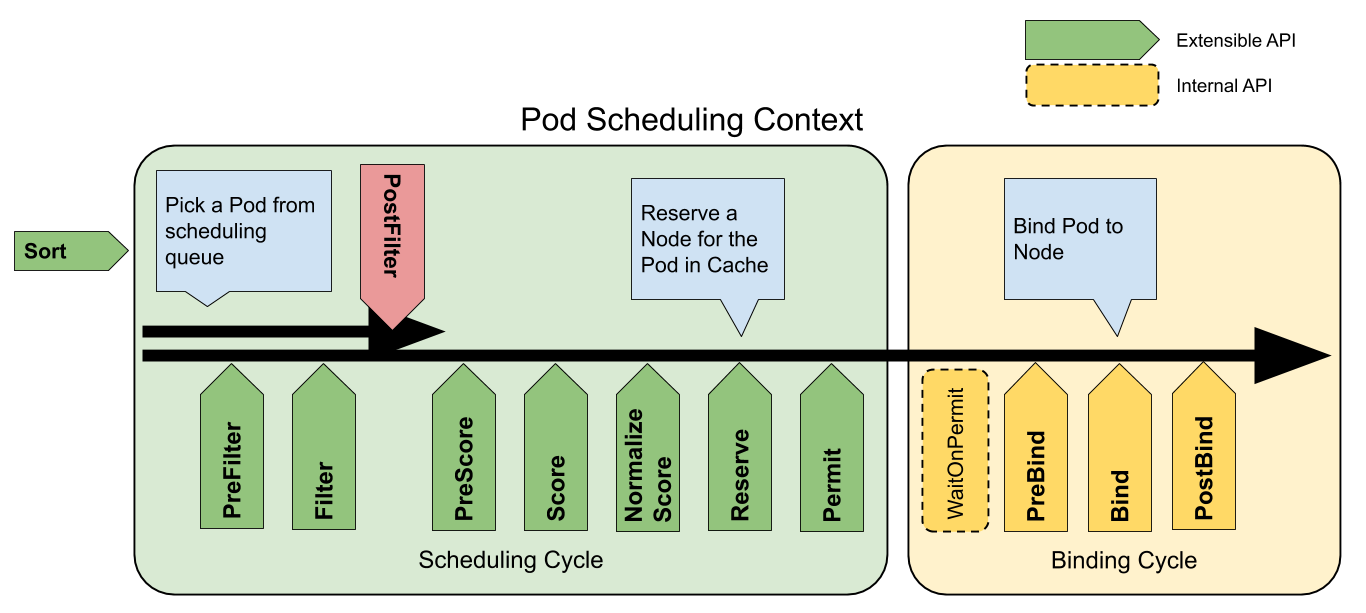
\includegraphics[width=\textwidth]{chapters/background/img/scheduler.png}
      \caption{The extension points of the scheduling framework}
      \label{fig:scheduling-plugins}
\end{figure}


\paragraph*{Scheduler framework extension points}

The scheduler framework offers the following extensions points where each plugin
can be registered:

\begin{itemize}
      \item
            \textbf{\co{Queue sort}}: The scheduler uses these plugins to sort
            Pods in the scheduling queue. A queue sort plugin essentially will
            provide a \co{less(pod1, Pod2)} function. Only one queue sort plugin
            may be enabled at a time.
      \item
            \textbf{\co{PreFilter}}: The scheduler uses these plugins to
            pre-process info about the Pod or to check certain conditions that
            the cluster or the Pod must meet. A PreFilter plugin should
            implement a \co{PreFilter} function. If \co{PreFilter} returns an
            error, the scheduler will abort the scheduling cycle..
      \item
            \textbf{\co{Filter}}: The scheduler uses these plugins to
            \textit{filter out} nodes that cannot run the Pod. For each node,
            the scheduler will call the filter plugins in their configured
            order. If any filter plugin marks the node as \textit{infeasible},
            the scheduler will not call the remaining plugins for that evaluated
            node. The scheduler may evaluate nodes concurrently, and thus, it
            may call a \co{Filter} plugin more than once in the same scheduling
            cycle.
      \item
            \textbf{\co{PostFilter}}: The scheduler calls these plugins in their
            configured order after the \co{Filter} phase, but only if it did not
            find any feasible nodes for the Pod. If any of them marks the node
            as schedulable, the scheduler will not call the remaining plugins. A
            typical PostFilter implementation is the \co{preemption} plugin,
            which tries to make the Pod schedulable by preempting other Pods.
      \item
            \textbf{\co{PreScore}}: This is an informational extension point for
            performing pre-scoring work. The scheduler will call the plugins
            with a list of nodes that passed the filtering phase. A plugin may
            use this data to update the internal state or to generate logs or
            metrics.
      \item
            \textbf{\co{Scoring}}: This extension point has two phases:
            \begin{itemize}
                  \item
                        The first phase is called ``\textit{score}'' and is used
                        to rank nodes that have passed the filtering phase. The
                        scheduler will call the \texttt{Score} method of each
                        scoring plugin for each node.
                  \item The second phase is ``\textit{normalize scoring}'' and
                        is used to modify scores before the scheduler computes a
                        final ranking of nodes.
            \end{itemize}

      \item
            \textbf{\co{Reserve}}: A plugin that implements the Reserve
            extension has two methods, namely \texttt{Reserve} and
            \texttt{Unreserve}. Plugins that maintain runtime state, i.e.,
            \textit{stateful plugins}, should use these phases to reserve and
            unreserve any resources in the internal state of the scheduler.

            The \emph{Reserve} phase exists to prevent race conditions while the
            scheduler waits for the bind to succeed. The scheduler executes it
            before it binds a Pod to its designated node. The \texttt{Reserve}
            method of each Reserve plugin may succeed or fail.

            If the \texttt{Reserve} method of all plugins succeeds, the
            scheduler considers the Reserve phase to be successful and executes
            the rest of the scheduling cycle and the binding cycle.

            If one \texttt{Reserve} method call fails, the scheduler will not
            execute the subsequent phases and will run the \co{Unreserve} phase
            instead. The \emph{Unreserve} phase exists to clean up the state
            associated with the reserved Pod. The scheduler calls the
            \co{Unreserve} method of all the \co{Reserve} plugins in the reverse
            order of \co{Reserve} method calls.
      \item
            \textbf{\co{Permit}}: The scheduler uses these plugins to prevent or
            delay the binding of a Pod. It executes them as the last step of a
            scheduling cycle; however, it waits for the permit phase to execute
            successfully at the beginning of a binding cycle, before executing
            the \texttt{PreBind} plugins.
\end{itemize}


\paragraph*{The \co{CycleState} struct}
\label{section:cycle-state}

The various plugins running in the scheduling context of a single Pod share a
common \co{CycleState} struct. \co{CycleState} provides a mechanism for plugins
to store and retrieve arbitrary data. Data stored in the \co{CycleState} by one
plugin can be read, altered, or deleted by another. \co{CycleState} does not
provide any data protection, as all plugins are assumed to be trusted.


\subsection{The VolumeBinding Plugin}\label{section:background_volume_binding}

The \texttt{VolumeBinding} plugin of the Kubernetes Scheduler binds Pod volumes
in scheduling. The VolumeBinding plugin is registered on the \texttt{PreFilter},
\texttt{Filter}, \texttt{PreBind}, \texttt{Reserve}, and \texttt{Unreserve}
extension points. The \texttt{PreFilter}, \texttt{Filter}, and \texttt{PreBind}
phases of the plugin are of particular interest in the context of this thesis.
We explain here briefly the operations that take place:

\begin{itemize}
      \tightlist
      \item \co{PreFilter}: Checks if a Pod has all its immediate (PVCs that
            request a storage class with \co{Immediate} binding mode) PVCs
            bound. If not all immediate PVCs are bound, the plugin returns an
            \co{UnschedulableAndUnresolvable} error.
      \item \co{Filter}:  Evaluates if a Pod fits a node due to the volumes it
            requests:
            \begin{itemize}
                  \tightlist
                  \item For \textit{bound PVCs}, it checks that the
                        corresponding node affinity of the PV of each PVC is
                        satisfied by the given node.
                  \item For each \textit{unbound PVC}, it tries to find an
                        available PVs that satisfies the PVC requirements
                        (access mode, requested capacity) and has node affinity
                        that matches the given node.
                  \item For each \co{unbound PVC} that did not find a matching
                        PV (hereafter referred to as the ``PVCs to provision''),
                        it checks if there is enough space on the node to
                        provision a volume.


                  \item The \co{Filter} method returns true if the following
                        conditions hold:
                        \begin{enumerate}
                              \item  he PVs the (bound) PVCs are bound to are
                                    accessible from the node
                              \item the unbound PVCs can be matched to an
                                    existing available PV that is accessible
                                    from the node or  have the storage driver
                                    dynamically provision such a PV, if there is
                                    enough storage.
                        \end{enumerate}

            \end{itemize}
      \item \co{PreBind}: PreBind updates the API Server with the assumed
            bindings and waits until the PersistentVolume controller has wholly
            finished the binding operation. If binding errors, times out or gets
            undone, then an error will be returned to retry scheduling.
\end{itemize}
